\documentclass{article}
\usepackage{blindtext}

\usepackage[top=1in, bottom=1in, left=1in, right=1in]{geometry}

\usepackage{amsmath}
\usepackage{graphicx}
\usepackage{commath}
\usepackage{siunitx}


\usepackage[b]{esvect}

\newcommand{\de}{\mathrm{d}}

\begin{document}
\title{Homework 5}
\author{Xueqi Li}
% \date{Feb 4, 2017}
% \email{xueqi.li@stonybrook.edu}

% \begin{abstract}
% Consider a vector (given with respect to a fixed Cartesian basis). Here $t$ means time.
% \[
% \vv{r}(t) = \sin(\pi t)\hat{x} + \cos(\pi t)\hat{y} - \sqrt{7}\hat{z}
% \]
% \end{abstract}

\maketitle

\begin{enumerate}
    \item Consider a potential energy in one dimension of the form
    \[
        U(r) = -\frac{A}{r} + \frac{1}{r^n}
    \]
    \begin{enumerate}
        \item Sketch this potential for the special value $A = \frac{1}{2}$, $n = 2$, i.e. $U(r) = -\frac{1}{2r} + \frac{1}{r^2}$
        \begin{center}
            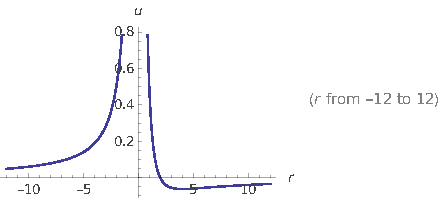
\includegraphics[height=1.5in]{plot.pdf}
        \end{center}

        \item For $r > 0$ and arbitrary $A > 0$, and any $n > 0$, what is the extremum $r_\text{eq}$ of this potential?\\

        \begin{align*}
            \frac{\de U}{\de r} &= 0\\
            \frac{\de }{\de r} \left[-A r^{-1} + r^{-n}\right] &= 0 \\
            A r^{-2} -n r^{n-1} &= 0\\
            \frac{A}{r^2} - \frac{n}{r^{n+1}} &= 0\\
            \frac{A}{r^2} &= \frac{n}{r^{n+1}} \\
            r^{n-1} &= \frac{n}{A}\\
            r &= \left(\frac{n}{A}\right)^{\frac{1}{n-1}}
        \end{align*}
        \item For this extremum $r_\text{eq}$, write the Taylor expansion for $U(r_\text{eq}+\delta)$ to second order in $\delta$.\\

        \begin{align*}
            U(r_\text{eq}+\delta) &= U(r_\text{eq}) + \frac{\de U}{\de r} (r_\text{eq}) \delta + \frac{1}{2}\frac{\de^2 U}{\de r^2} (r_\text{eq}) \delta^2 + \cdots\\
            &\approx  U(r_\text{eq}) + \frac{\de U}{\de r} (r_\text{eq}) \delta + \frac{1}{2}\frac{\de^2 U}{\de r^2} (r_\text{eq}) \delta^2 \\
        \end{align*}
        and we can find
        \begin{align*}
            &U(r_\text{eq}) = -A (\frac{A}{n})^\frac{1}{n-1} + (\frac{A}{n})^\frac{n}{n-1}\\
            &\frac{\de U}{\de r} (r_\text{eq}) = 0 \\
            &\frac{\de^2 U}{\de r^2} = -2 Ar^{-3} + n^2 r^{-n-2} + nr^{-n-2} \\
            &\frac{\de^2 U}{\de r^2} (r_\text{eq}) = -2 A(\frac{A}{n})^\frac{3}{n-1} + n^2 (\frac{A}{n})^\frac{n+2}{n-1} + n(\frac{A}{n})^\frac{n+2}{n-1}
        \end{align*}
        Wwhich give us:
        \begin{align*}
            U(r_\text{eq}+\delta) \approx 
                \left[-A (\frac{A}{n})^\frac{1}{n-1} + (\frac{A}{n})^\frac{n}{n-1}\right]\delta
                +\frac{1}{2}\left[-2 A(\frac{A}{n})^\frac{3}{n-1} + n^2 (\frac{A}{n})^\frac{n+2}{n-1} + n(\frac{A}{n})^\frac{n+2}{n-1}\right]\delta^2
        \end{align*}
        if we chose $r_\text{eq}$ as the reference point, thus we have
        \[
            U = \frac{1}{2}\left[-2 A(\frac{A}{n})^\frac{3}{n-1} + n^2 (\frac{A}{n})^\frac{n+2}{n-1} + n(\frac{A}{n})^\frac{n+2}{n-1}\right]\delta^2
        \]
        \item If the particle has a mass $m$, what is the angular frequency of small oscillations?\\

        For $U$ we have:
        \begin{align*}
            U &= \frac{1}{2}kx^2 \\
            \frac{\de U}{\de x} &= kx \\
            \frac{\de^2 U}{\de x^2} &= k
        \end{align*}
        Thus we have $k$ as:
        \[
        k = \frac{1}{2}[-2 A(\frac{A}{n})^\frac{3}{n-1} + n^2 (\frac{A}{n})^\frac{n+2}{n-1} + n(\frac{A}{n})^\frac{n+2}{n-1}]
        \]
        Thus we have
        \[
        \omega = \sqrt{\frac{k}{m}} = \sqrt{\frac{1}{2}\left[-2 A(\frac{A}{n})^\frac{3}{n-1} + n^2 (\frac{A}{n})^\frac{n+2}{n-1} + n(\frac{A}{n})^\frac{n+2}{n-1}\right] \frac{1}{m}}
        \]

    \end{enumerate}
    \item The mass shown from above in figure is resting on a friction less horizontal table. Each of the two identical springs has force constant $k$ and unstretched length $l_0$. At equilibrium the mass rests at the origin, and the distances $a$ are not necessarily equal to $l_0$. (That is, the springs may already be stretched or compressed.) Show that when the mass moves to a position $(x,y)$, with $x$ and $y$ small, the potential energy has the form for an anisotripic oscillator. Show that if $a < l_0$ the equilibrium at the origin is unstable and explain why.
    \[
    U = \frac{1}{2}(k_xx^2 + k_yy^2)
    \]\\

    we have for $r$:
    \[
    \left\{
    \begin{aligned}
    r_1 = \sqrt{y^2 + (a+x)^2} \\
    r_2 = \sqrt{y^2 + (a-x)^2}
    \end{aligned}
    \right. 
    \] 

    For the force, we have:
    \[
    \left\{
    \begin{aligned}
    F_1 = -k(r_1 - l_0) \\
    F_2 = -k(r_2 - l_0)
    \end{aligned}
    \right. 
    \] 
    And we find $F_x$ and $F_y$ from it:
    \[
    \left\{
    \begin{aligned}
    F_x &= -k(r_1-l_0)\frac{x+a}{r_1} - k(r_2 - l_0)\frac{a-x}{r_2} \\
    F_y &= -k(r_1-l_0)\frac{y}{r_1} - k(r_2-l_0)\frac{y}{r_2}
    \end{aligned}
    \right. 
    \] 

    Now we want to find the energy. If we Taylor expand the energy near the equilibrium point, which is choose as $(0,0)$ here, we have:
    \[
    U = U(0,0) + \frac{\de U}{\de \vv{r}}(0,0) \vv{r} + \frac{1}{2}\frac{\de^2 U}{\de \vv{r}} (0,0)\vv{r}^2 + \cdots
    \]
    now notice that since we chose the equilibrium point as $(0,0)$, $U(0,0) = 0$. Moreover, since this is an equilibrium point, $\frac{\de U}{\de \vv{r}} = 0$. Thus we have:
    \[
    U \approx \frac{1}{2}\frac{\de^2 U}{\de \vv{r}} (0,0)\vv{r}^2
    \]
    Also we can notice that $U = \int F \cdot \de \vv{r}$. Thus we have:
    \[
    U \approx \frac{\de F}{\de \vv{r}}(0,0) \vv{r}^2
    \]

    Thus we have:
    \[
    \left\{
    \begin{aligned}
    F_x &= -k(\sqrt{y^2 + (a+x)^2}-l_0)\frac{x+a}{\sqrt{y^2 + (a+x)^2}} - k(\sqrt{y^2 + (a-x)^2} - l_0)\frac{a-x}{\sqrt{y^2 + (a-x)^2}} \\
    F_y &= -k(\sqrt{y^2 + (a+x)^2}-l_0)\frac{y}{\sqrt{y^2 + (a+x)^2}} - k(\sqrt{y^2 + (a-x)^2}-l_0)\frac{y}{\sqrt{y^2 + (a-x)^2}}
    \end{aligned}
    \right. 
    \] 
    Thus we have:
    \begin{align*}
        \frac{\de F_x}{\de x} =& -\frac{k (a - x)^2 \sqrt{(a - x)^2 + y^2} - l}{((a - x)^2 + y^2)^\frac{3}{2}} \\\
        &+ \frac{k (\sqrt{(a - x)^2 + y^2} - l)}{\sqrt{(a - x)^2 + y^2}} \\
        &- \frac{k (\sqrt{(a + x)^2 + y^2} - l)}{\sqrt{(a + x)^2 + y^2}} \\
        &+ \frac{k (a + x)^2 (\sqrt{(a + x)^2 + y^2} - l)}{((a + x)^2 + y^2)^\frac{3}{2}} \\
        &+ \frac{k (a - x)^2}{((a - x)^2 + y^2)} \\
        &- \frac{k (a + x)^2}{((a + x)^2 + y^2)}
    \end{align*}
    and we evaluate it at $(0,0)$:
    \begin{align*}
        \frac{\de F_x}{\de x}(0,0) &= -\frac{k a^2 a - l}{a^3} 
        + \frac{k (a - l)}{a} 
        - \frac{k (a - l)}{a} 
        + \frac{k a^2 (a - l)}{a^3} 
        + \frac{k a^2}{a^2} 
        - \frac{k a^2}{a^2} \\
        &= -\frac{k a^2 (a - l)}{a^3} 
        + \frac{k a^2 (a - l)}{a^3} =0
    \end{align*}
    Thus we take $k_x = 0$ as $k_x = \iint U \de x$ as $U = \frac{1}{2}k_xx$.

    And we have

    And for $y$:
    \begin{align*}
        \frac{\de F_y}{\de y} = 
        &\frac{k y^2 (\sqrt{(a - x)^2 + y^2} - l)}{(a - x)^2 + y^2)^(3/2)}\\
        &+ \frac{k y^2 (\sqrt{(a + x)^2 + y^2} - l)}{(a + x)^2 + y^2)^(3/2)} \\
        &- \frac{k (\sqrt{(a - x)^2 + y^2} - l)}{\sqrt{(a - x)^2 + y^2} }\\
        &- \frac{k (\sqrt{(a + x)^2 + y^2} - l)}{\sqrt{(a + x)^2 + y^2} }\\
        &- \frac{k y^2}{(a - x)^2 + y^2} \\
        &- \frac{k y^2}{(a + x)^2 + y^2)}
    \end{align*}
    And we have:
    \begin{align*}
        \frac{\de F_y}{\de y} (0,0) = - 2\frac{k (a - l)}{a}\\
    \end{align*}
    Thus we have:
    \[
        U_y \approx = -\frac{k (a - l)}{a}y^2
    \]
    Moreover, we have
    \[
        k_y =  -\frac{2k (a - l)}{a}
    \]
    where $k_y = \iint U \de y$ as $U = \frac{1}{2}k_yy$.

    Thus we have 
    \[
    U = \frac{1}{2}(k_x^2+k_y^2)
    \]

    When $a < l$, easy to see that $\frac{\de^2 U}{\de^2 y}>0$ from above result, which gives a velocity to the mass, i.e., when $a < l$, $U$ is maximum value, any tiny displacement will make move further away from the equilibrium point.

    % thus, we have energy as:
    % \begin{align*}
    %     U &= \frac{1}{2} k (r_1 - l_0)^2 + \frac{1}{2} k (r_2 - l_0)^2\\
    % \end{align*}



    \item An undamped oscillator has period $T$. A bit of damping is added, and the period changes to $T\sqrt{1+q^2}$, where $q$ is some constant.
    \begin{enumerate}
        \item What is the damping factor $\beta$? What is the quality factor $Q$? \\

        From the problem we have:
        \[
        T = \frac{2\pi}{\omega_0} \, , \, T' = T\sqrt{1+q^2} = \frac{2\pi}{\omega_0}\sqrt{1+q^2} = \frac{2\pi}{\omega}
        \]
        Thus from $T'$ we can find
        \begin{align*}
            \omega_0 = \omega\sqrt{1+q^2} \\
            \omega_0^2 = \omega^2(1+q^2)
        \end{align*}
        Notice that
        \begin{align*}
            \omega^2 &= \omega_0^2 - \beta^2 \\
            \beta^2 &= \omega_0^2 - \omega^2 \\
            \beta^2 &= \omega^2(1+q^2) - \omega^2 \\
            \beta^2 &= \omega(1+q^2-1)\\
            \beta^2 &= \omega^2 q^2\\
            \beta &= \omega q
        \end{align*}
        and for quality factor:
        \[
        Q = \frac{\omega}{2\beta} = \frac{\omega}{2\omega q} = \frac{1}{q}
        \]
        \item Suppose $q = \frac{1}{2\pi}$. What is the percentage change in the angular frequency? Approximately how many cycles are needed before the amplitude drops by a factor of $e$? Which effect is more noticeable?\\

        From above, we have
        \begin{align*}
            \frac{\omega}{\omega_0} = \frac{1}{\sqrt{1+q^2}} = \frac{1}{\sqrt{1+\frac{1}{4\pi^2}}} = 0.9876
        \end{align*}

        \begin{align*}
            e^{-MT'\beta} &= \frac{1}{e} \\
            MT'\beta &= 1 \\
            M &= \frac{1}{\beta T'} \\
            M &= \frac{1}{\omega q T} \\
            M &= \frac{\omega}{\omega q 2\pi} \\
            M &= \frac{1}{q 2\pi}\\
            M &= \frac{2\pi}{2\pi} \\
            M &= 1
        \end{align*}

    \end{enumerate}
    \item Consider an overdamped harmonic oscillator with a driving force $F_\omega \sin(\omega_F t)$.
    \begin{enumerate}
        \item Find the motion without transients.\\

        We could chose the $t= 0$ so that we have the driving force as $F \cos(\omega t)$. This just make a time shift of hour resould, which does not matter since the system is periodic. Thus we can write the force as $F e^{i\omega t}$.
        Given differential equation:
        \[
        \ddot{x} + 2\beta \dot{x} + \omega_0^2 x = \frac{F}{m} e^{i\omega t}
        \]
        such a differential equation have two solution, where the final solution is a linear combination of the two solution. Now we know that the solution have a form:
        \[
        x = Ae^{i(\omega t - \varphi)}
        \]
        Now we just plug it into the equation:
        \begin{align*}
            \ddot{x} + 2\beta \dot{x} + \omega_0^2 x &= \frac{F}{m} e^{i\omega t}\\
            -A \omega^2 e^{i(\omega t - \varphi)} + 2\beta A i \omega e^{i(\omega t - \varphi)} + \omega_0^2 A e^{i(\omega t - \varphi)} &= \frac{F}{m}e^{i\omega t}\\
            (-\omega^2+2\beta \omega i + \omega_0^2) A e^{i(\omega t - \varphi)} &= \frac{F}{m}e^{i\omega t} \\
            (-\omega^2+2\beta \omega i + \omega_0^2) A &= \frac{F}{m} e^{i \varphi} \\
            (-\omega^2+2\beta \omega i + \omega_0^2) A &= \frac{F}{m} (\cos\varphi + i \sin \varphi)
        \end{align*}
        To solve this we can first separate the real and the imaginary part:
        \[
        \left\{
        \begin{aligned}
        ( -\omega^2+\omega_0^2)A = \frac{F}{m} \cos\varphi \\
        2\beta \omega A = \frac{F}{m} \sin \varphi
        \end{aligned}
        \right. 
        \] 
        Thus, we could have:
        \begin{align*}
            \frac{\sin\varphi}{\cos\varphi} = \frac{2\beta \omega}{ -\omega^2+\omega_0^2} \\
            \tan \varphi= \frac{2\beta \omega}{ -\omega^2+\omega_0^2}
        \end{align*}
        Or we could have
        \begin{align*}
            (-\omega^2+2\beta \omega i + \omega_0^2) A &= \frac{F}{m} e^{i \varphi}\\
            (-\omega^2+2\beta \omega i + \omega_0^2)(-\omega^2+2\beta \omega i + \omega_0^2)^* A A^* &= \frac{FF^*}{mm^*} e^{i \varphi}e^{i \varphi}* \\
            [(\omega_0^2-\omega^2)+4\beta^2 \omega^2]A^2 &= \frac{F^2}{m^2}\\
            A^2 &= \frac{F^2}{m^2}\frac{1}{(\omega_0^2-\omega^2)+4\beta^2 \omega^2} \\
            A &= \frac{F}{m}\frac{1}{\sqrt{(\omega_0^2-\omega^2)+4\beta^2 \omega^2}}
        \end{align*}


        \item Find the motion if the initial position and velocity vanish.\\

        We want to find a solution such that $x(0) = \dot{x}(0) = 0$. Thus we have $x = Ae^{-i\varphi}$. Plug it into the equation:
        \begin{align*}
            \ddot{x} + 2\beta \dot{x} + \omega_0^2 x &= \frac{F}{m} e^{i\omega t} \\
            -A\omega^2 e^{-i\varphi}  &= \frac{F}{m}\\
            -A\omega^2 &= \frac{F}{m} e^{i\varphi}\\
            -A\omega^2 &= \frac{F}{m} (\cos\varphi + i \sin\varphi)
        \end{align*}
        Now we find that the imaginary part is zero in the left side:
        \begin{align*}
            \sin\varphi &= 0 \\
            \varphi &= 0 \,\, \text{or} \,\,\pi
        \end{align*}
        Thus we have
        \begin{align*}
            -A\omega^2 &= \pm \frac{F}{m} \\
            A &= \mp \frac{F}{m} \frac{1}{\omega^2}
        \end{align*}

        Now if we want to solve it without the time shift, we can have:
        \begin{align*}
            -A\omega^2 e^{-i\varphi}  &= \frac{F}{m} e^{-i\frac{\pi}{2\omega}} \\
            -A\omega^2 &= \frac{F}{m} e^{i(\varphi - \frac{\pi}{2\omega})} \\
            -A\omega^2 &= \frac{F}{m} \cos(\varphi - \frac{\pi}{2\omega}) + i \cos(\varphi)
        \end{align*}
        Thus we have $\cos(\varphi) = 0$, which give us $\varphi = \frac{\pi}{2}$ or $\frac{3\pi}{2}$. Thus we have:
        \begin{align*}
            -A\omega^2 &= \frac{F}{m} \cos(\varphi - \frac{\pi}{2\omega}) \\
            -A\omega^2 &= \frac{F}{m} \sin(\varphi)\\
            -A\omega^2 &= \pm\frac{F}{m} \\
        \end{align*}
        Which give our same result as above. The only difference is a $\frac{T}{4}$ phase shift.


    \end{enumerate}
    \item Consider a RLC circuit with a resistor with resistance $R$ in series with a capacitor with capacitance $C$ and an inductor with inductance $L$.
    \begin{enumerate}
        \item What is the natural frequency $\omega$ and what is the damping factor $\beta$? \\

        We have following equation for LRC:
        \begin{align*}
            &V_R = IR = \dot{Q}R\\
            &V_L = L\dot{I} = \ddot{Q}L\\
            &V_C = \frac{Q}{C}
        \end{align*}
        Now since thsere is not input to the circuit, we have $V = 0$, which gives us:
        \[
        \ddot{Q}L + \dot{Q}R + \frac{Q}{C} = 0
        \]
        where now we can change this to stander euqation of oscillations:
        \[
        \ddot{Q} + 2\beta\dot{Q} + \omega_0^2Q = 0 \,\,\,\,\, \text{where}\,\, \beta = \frac{R}{2L}\,\,,\,\,\omega_0 = \sqrt{\frac{1}{LC}} 
        \] 
        and we have
        \[
        \omega = \sqrt{\omega_0^2 - \beta^2}
        \]
        \item Suppose this is being driven by a voltage $V(t) = A \cos(\frac{\omega}{2}t) + B\sin(2\omega t)$. \\

        From the driving force we have:
        \[
        \ddot{Q} + 2\beta\dot{Q} + \omega_0^2Q = A \cos(\frac{\omega}{2}t) + B\sin(2\omega t)
        \]
        since $(D^2 + 2\beta D + \omega_0^2 I)$ is a linear operator as differential operation is linear. Thus the solution of above equation is just a linear combination of
        \[
        \left\{
        \begin{aligned}
        \ddot{Q} + 2\beta\dot{Q} + \omega_0^2Q = A \cos(\frac{\omega}{2}t)\\
        \ddot{Q} + 2\beta\dot{Q} + \omega_0^2Q = B\sin(2\omega t)
        \end{aligned}
        \right. 
        \] 
        Thus the solution is just:
        \[
        Q = A C_A \cos(\frac{\omega}{2}t - \varphi_A) + B C_B \sin(2\omega t - \varphi_B)
        \]
        where
        \[
        C_A = \frac{1}{\sqrt{(\omega_0^2 - (\frac{\omega}{2})^2)^2 + \beta^2\omega^2}}
        \]
        and
        \[
        C_B = \frac{1}{\sqrt{(\omega_0^2 - 4\omega^2)^2 + 16\beta^2\omega^2}}
        \]
        To find the circuit, than we have:
        \[
        I = \dot{Q} = - \frac{1}{2} A \omega C_A \sin(\frac{\omega}{2}t - \varphi_A) + 2 B \omega C_B \cos(2\omega t - \varphi_B)
        \]

    \end{enumerate}
\end{enumerate}
      




% \begin{eqnarray*}
\end{document}